Nella soluzione hardware in questione verrà utilizzata la direttiva di pipeline, di unrolling di fattore pari a 2 e la direttiva di partizionamento di tipologia cyclic. Nello specifico, verranno analizzate le seguenti implementazioni relative al loop2:
\begin{itemize}
	\item Pipeline, Unroll=2, Cyclic=8 (columnIndex, values, x)
	\item Pipeline, Unroll=2, Cyclic=8 (columnIndex)
	\item Pipeline, Unroll=2, Cyclic=8 (values)
	\item Pipeline, Unroll=2, Cyclic=8 (x)
\end{itemize}

In particolare, è possibile evidenziare nel dettaglio le differenti soluzioni hardware nei seguenti allegati.
\lstinputlisting[language=C++]{solutions/s10/s10all3.cpp}
\lstinputlisting[language=C++]{solutions/s10/s10columnIndex.cpp}
\lstinputlisting[language=C++]{solutions/s10/s10values.cpp}
\lstinputlisting[language=C++]{solutions/s10/s10x.cpp}

Effettuando la sintesi si ottiene il seguente log.
\\
\textcolor{red}{ERROR: [XFORM 203-103] Cannot partition array 'x' (smvmProject/smvm.cpp:11): incorrect partition factor 8.}
\\
In particolare, la console sta segnalando che effettivamente non riesce a partizionare l'array x dal momento che la dimensione dell'array risulta essere non compatibile con il fattore di partitioning dichiarato. Infatti, la dimensione di x inizialmente dichiarata in definitions.h è pari a 4 mentre il fattore di partizionamento che si sta utilizzando è pari a 8. A questo proposito si potrebbe modificare il valore di dimensionamento relativo a x all'interno dell'header. In particolare è necessario modificare sia il valore di size sia il valore di rows. Inoltre, bisogna anche modificare i parametri dichiarati all'interno della direttiva trip count dal momento che il numero di righe e, quindi, di iterazioni risulta essere differente.
\lstinputlisting[language=C]{solutions/s10/headermodified.h}
\lstinputlisting[language=C++]{solutions/s10/s10all3modified.cpp}
\lstinputlisting[language=C++]{solutions/s10/s10columnIndexmodified.cpp}
\lstinputlisting[language=C++]{solutions/s10/s10valuesmodified.cpp}
\lstinputlisting[language=C++]{solutions/s10/s10xmodified.cpp}

Pertanto, effettuando la sintesi si ottiene il seguente report.

\begin{table}[H]
	\centering
	\begin{tabular}{|c|c|c|c|c|}
		\hline
		\textbf{Solution} & \textbf{Clock} & \textbf{Target} & \textbf{Estimated} & \textbf{Uncertainty} \\
		\hline
		columnIndex, values, x & ap\_clk & 10.00 & 8.510 & 1.25 \\
		\hline
		columnIndex & ap\_clk & 10.00 & 8.510 & 1.25 \\
		\hline
		values & ap\_clk & 10.00 & 8.510 & 1.25 \\
		\hline
		x & ap\_clk & 10.00 & 8.510 & 1.25 \\
		\hline
	\end{tabular}
	\caption{HLS Solution 10 Timing Summary (ns)}
	\label{tab:hls-solution-10-timing-summary}
\end{table}

\begin{table}[H]
	\centering
	\begin{tabular}{|c|c|c|c|c|}
		\hline
		\multicolumn{1}{|c|}{\textbf{Solution}} & \multicolumn{2}{|c|}{\textbf{Latency}} & \multicolumn{2}{|c|}{\textbf{Interval}} \\
		& min & max & min & max \\
		\hline
		columnIndex, values, x & 57 & 89 & 57 & 89 \\
		\hline
		columnIndex & 65 & 97 & 65 & 97 \\
		\hline
		values & 65 & 97 & 65 & 97 \\
		\hline
		x & 57 & 89 & 57 & 89 \\
		\hline
	\end{tabular}
	\caption{HLS Solution 10 Latency Summary (clock cycles)}
	\label{tab:hls-solution-10-latency-summary}
\end{table}

\begin{table}[H]
	\centering
	\begin{tabular}{|c|c|c|c|c|c|c|c|c|c|}
		\hline
		\multicolumn{1}{|c|}{\textbf{Solution}} & \multicolumn{1}{|c|}{Loop Name} & \multicolumn{2}{|c|}{\textbf{Latency}} & \multicolumn{1}{c|}{\textbf{Iteration Latency}} & \multicolumn{2}{c|}{\textbf{Initiation Interval}} & \multicolumn{1}{c|}{\textbf{Trip}}  \\
		&  & min & max & & achieved & target & \textbf{Count} \\
		\hline
		columnIndex, values, x & - loop1 & 56 & 88 & 7$\sim$11 & - & - & 8 \\
		& + loop2 & 3 & 7 & 4 & 1 & 1 & 0$\sim$4 \\
		\hline
		columnIndex & - loop1 & 64 & 96 & 8$\sim$12 & - & - & 8 \\
		& + loop2 & 4 & 8 & 5 & 1 & 1 & 0$\sim$4 \\
		\hline
		values & - loop1 & 64 & 96 & 8$\sim$12 & - & - & 8 \\
		& + loop2 & 4 & 8 & 5 & 1 & 1 & 0$\sim$4 \\
		\hline
		x & - loop1 & 56 & 88 & 7$\sim$11 & - & - & 8 \\
		& + loop2 & 3 & 7 & 4 & 1 & 1 & 0$\sim$4 \\
		\hline
	\end{tabular}
	\caption{HLS Solution 10 Latency Loops Summary }
	\label{tab:hls-solution-10-loop-summary}
\end{table}

\begin{table}[H]
	\centering
	\begin{tabular}{|c|c|c|c|c|}
		\hline
		\textbf{Solution} & \textbf{BRAM\_18K} & \textbf{DSP48E} & \textbf{FF} & \textbf{LUT} \\
		\hline
		columnIndex, values, x & 0 & 6 & 762 & 900 \\
		\hline
		columnIndex & 0 & 6 & 539 & 752 \\
		\hline
		values & 0 & 6 & 640 & 773 \\
		\hline
		x & 0 & 6 & 727 & 492 \\
		\hline
	\end{tabular}
	\caption{HLS Solution 10 Utilization Estimates [\#]}
	\label{tab:hls-solution-10-utilization-report}
\end{table}

\begin{figure}[H]
	\centering
	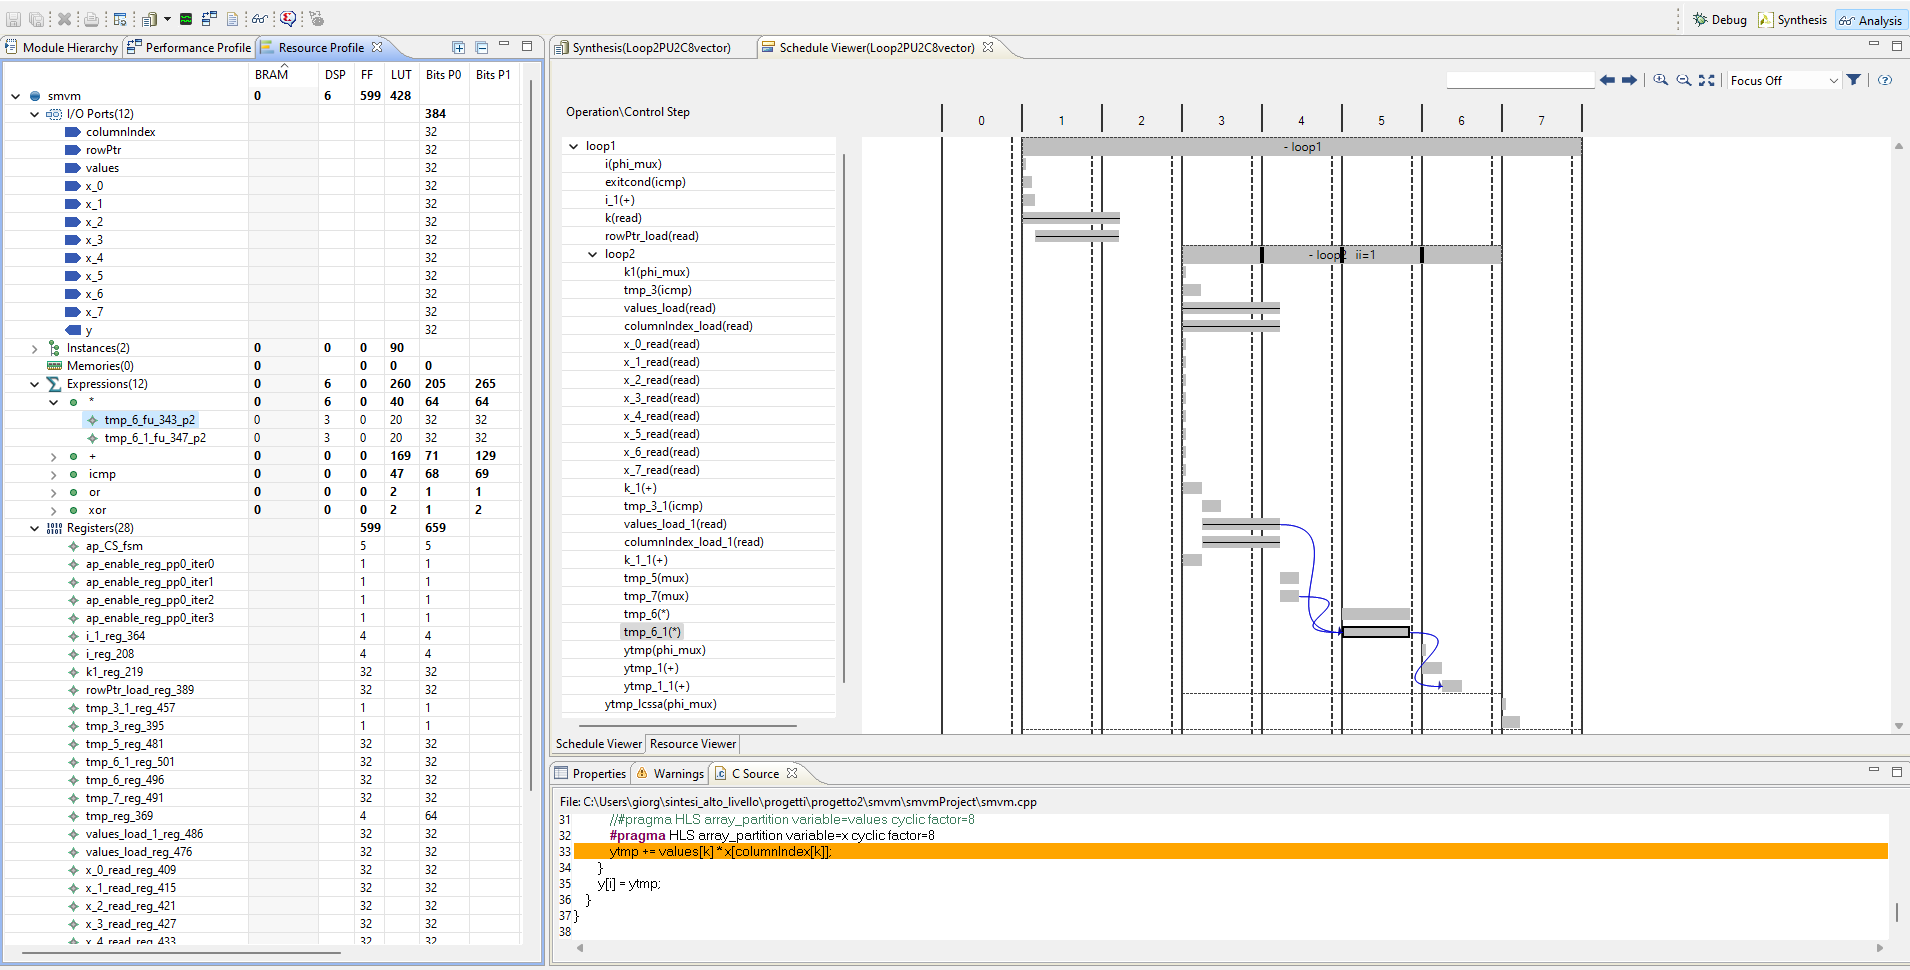
\includegraphics[width=0.9\textwidth]{solutions/s10/s10analysis.png}
	\caption{HLS Solution 10 Analysis}
\end{figure}

In particolare, dall'interfaccia Analysis sotto allegata (corrispondente al partitioning dell'array x), si può notare come l'unrolling di fattore 2 sia stato applicato correttamente dal momento che vengono effettuate 2 operazioni di moltiplicazione e 2 operazioni di somma in un'unica iterazione del loop2. Nello specifico, si può evidenziare come i prodotti richiedano l'utilizzo di 3 DSP ognuno tale da giustificare l'utilizzazione di tali risorse pari a 6 come riportato nel report di sintesi. 

\begin{table}[H]
	\centering
	\begin{tabular}{|c|c|c|c|c|c|c|c|c|}
		\hline
		\multicolumn{1}{|c|}{\textbf{Solution}} & \multicolumn{1}{|c|}{RTL} & \multicolumn{1}{|c|}{Status} & \multicolumn{3}{c|}{\textbf{Latency}} & \multicolumn{3}{c|}{\textbf{Interval}} \\
		& &  & min & avg & max & min & avg & max \\
		\hline
		columnIndex, values, x & VHDL & Pass & 61 & 61 & 61 & NA & NA & NA \\
		\hline
		columnIndex & VHDL & Pass & 69 & 69 & 69 & NA & NA & NA \\
		\hline
		values & VHDL & Pass & 69 & 69 & 69 & NA & NA & NA \\
		\hline
		x & VHDL & Pass & 61 & 61 & 61 & NA & NA & NA \\
		\hline
	\end{tabular}
	\caption{HLS Solution 10 C/RTL Cosimulation Report }
	\label{tab:hls-solution-10-cosimulation-report}
\end{table}

Si può notare come l'utilizzazione delle risorse sia aumentata rispetto alle soluzioni 6 (loop2 Pipeline, Unroll=2, Cyclic=2) e 8 (loop2 Pipeline, Unroll=2, Cyclic=4). In particolare, considerando le soluzioni hardware corrispondenti al partizionamento di tutti e tre gli array, si evidenzia rispettivamente un aumento di circa l'$81\%$ e di circa il $66\%$ in corrispondenza delle slice rispetto alla soluzione 6 e 8, un aumento di circa il $77\%$ e di circa il $63\%$ in corrispondenza delle LUT, un aumento di circa il $127\%$ e di circa il $43\%$. 
\\
Per quanto riguarda le soluzioni hardware corrispondenti al partizionamento di columnIndex, rispetto alla soluzione 6 e 8, si registra rispettivamente un aumento di un'unità e una diminuzione di 2 slice, un aumento di nove unità e di 7 unità delle LUT, un aumento di 6 unità e di 4 unità dei FF. 
\\
Per quanto riguarda le solution corrispondenti al partitioning di values, rispetto alla soluzione 6 e 8, si registra rispettivamente un aumento di circa il $18\%$ e di circa il $27\%$ delle slice, un aumento di 15 unità e di circa il $25\%$ delle LUT, una diminuzione di 25 unità e un aumento di 3 unità dei FF. 
\\
Per quanto riguarda le soluzioni hardware corrispondenti al partizionamento di x, rispetto alla soluzione 6 e 8, si registra rispettivamente un aumento di circa il $44\%$ e di circa il $38\%$ delle slice, un aumento di circa il $24\%$ e di circa il $25\%$ delle LUT, un aumento di circa il $124\%$ e di circa il $42\%$ dei FF.

\begin{table}[H]
	\centering
	\begin{tabular}{|c|c|c|c|c|c|c|c|c|}
		\hline
		\textbf{Solution} & \textbf{SLICE} & \textbf{LUT} & \textbf{FF} & \textbf{DSP} & \textbf{BRAM} & \textbf{CP} & \textbf{CP} & \textbf{CP} \\
		& & & & & & \textbf{required} & \textbf{achieved} & \textbf{achieved}\\
		& & & & & & & \textbf{post-} & \textbf{post-}\\
		& & & & & & & \textbf{synthesis} & \textbf{implementation}\\
		\hline
		columnIndex, values, x  & 204 & 558 & 449 & 6 & 0 & 10 & 6.540 & 6.840 \\
		\hline
		columnIndex  & 83 & 268 & 230 & 6 & 0 & 10 & 7.496 & 8.115 \\
		\hline
		values  & 117 & 342 & 199 & 6 & 0 & 10 & 7.927 & 7.603 \\
		\hline
		x  & 143 & 311 & 444 & 6 & 0 & 10 & 6.540 & 6.790 \\
		\hline
	\end{tabular}
	\caption{HLS Solution 10 Export RTL Report}
	\label{tab:hls-solution-10-export-rtl-report}
\end{table}

Ovviamente questo aumento di utilizzazione delle risorse è dovuto all'incremento del fattore di partizionamento adottato nelle soluzioni hardware. Infatti, si evidenzia che il maggiore incremento delle risorse si ha rispetto alla soluzione 6 dove era previsto un fattore pari a 2 rispetto alla soluzione in questione dove il fattore di partitioning previsto è stato di 8.